\chapter{前期活動内容}
第4章ではグループBの活動内容について紹介する。活動していく中で、意識した点や失敗した要因、その中で身についたことに関して記述している。
\section{完成の理想についての議論}
% 担当:小山内魁人
グループBでは、結成当初、北海道新聞のデータを利用できることから、それを生かした北海道すごろくゲームを考案した。このゲームは適切な新聞記事をユーザに読ませるマスやミニゲームを行うマスでポイントを競い合うことを想定していた。
また、このゲームは新聞記事データを用いることが目的になっていた。しかし、これらは現状の問題を発見しそれを解決することが目的になっておらず、この成果物はシステム情報科学実習の一環として行うことが不適切であると判断した。その後、目的と成果物の整合性がとれるように話し合った。
\bunseki{小山内魁人}
\section{新聞の現状の理解}
% 担当:金澤快飛
4.1で各グループメンバでの成果物案を出し合ったが、企画を実現するにあたって必要な根拠が不確かであった。そこで、各々が調査してきた新聞の現状をGoogle Jamboard内で情報共有し、集約する工程を行った。Google Jamboardとは、Googleが提供する、リアルタイムで共同作業が可能なホワイトボードのことである(図4.1)。初期の段階では、情報共有ノートの役割を果たすScrapboxを利用していたが、文字の書き込み以外に適していないという問題があった。そこで、オンラインでの活動が多かったこともあり、リアルタイム性が高く、文字や図を自由に書き込めるこのシステムを利用するに至った。\\
 情報共有の場では、新聞の購読率の低下が見られ、特に若者の購読者が少ないことがわかった。その理由としては、購読料が高い、インターネットのような他の媒体がある、読む時間が取れないなどの意見が挙げられた。一方、スマートフォンやゲームの利用率が一番高いのは若者であることから、新聞とゲームを組み合わせるきっかけとなった。話し合いを進める中で北海道新聞函館支社長の三浦辰治さんから、アメリカのニューヨークにある新聞社の The New York Times では、電子版の新聞にクロスワードパズルを導入したことにより、購読者数を増加させたという話を聞いた。
\newpage
\begin{figure}[htbp]
    \centering
    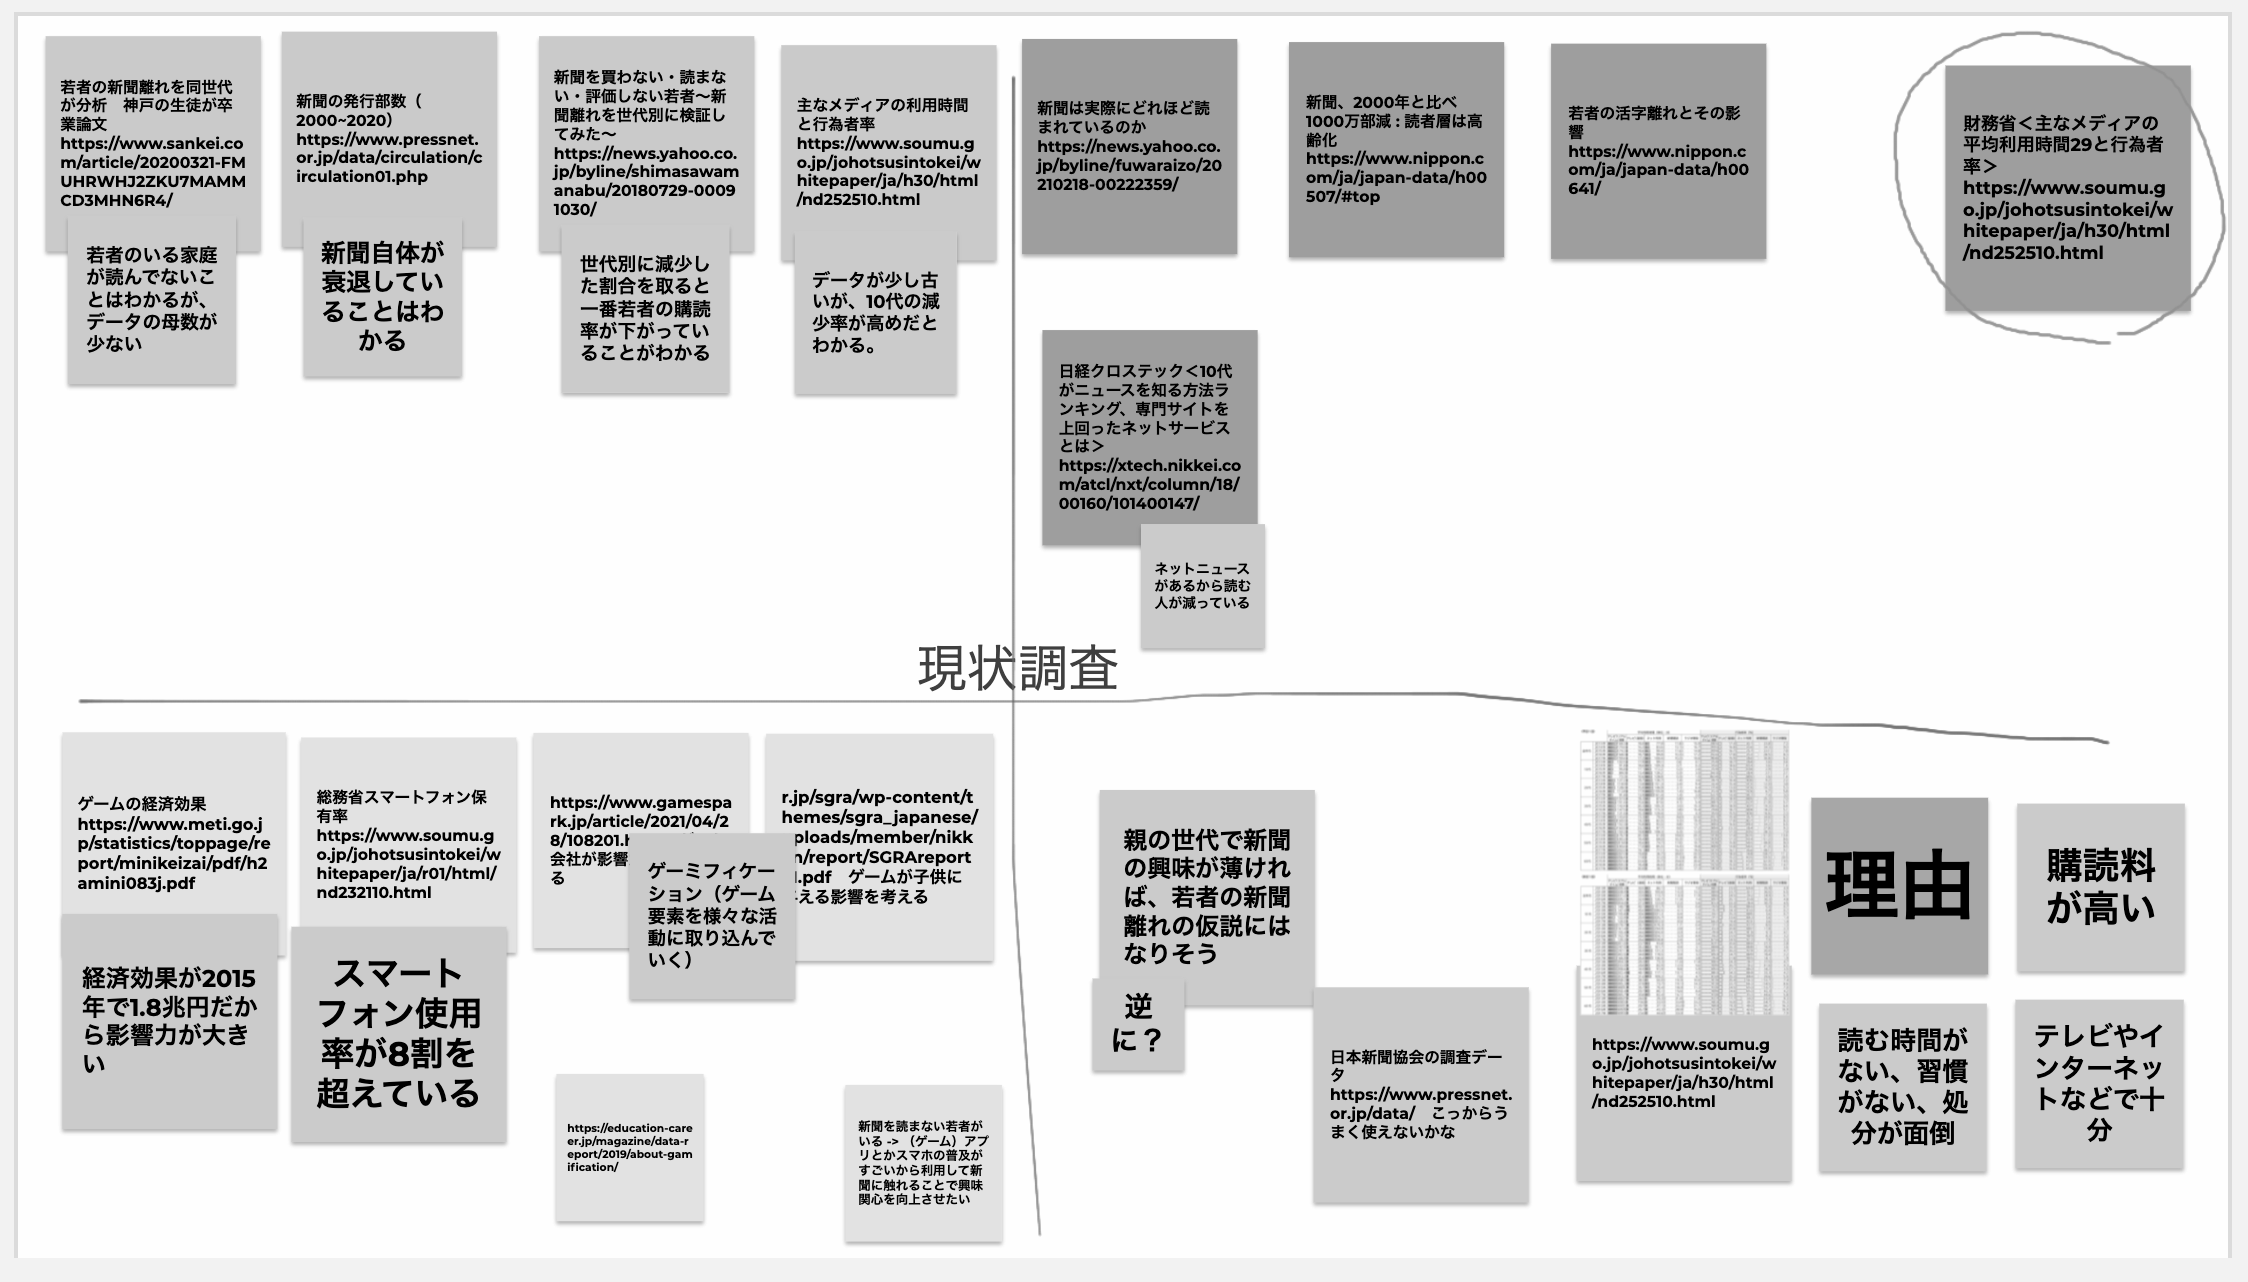
\includegraphics[width=12cm]{images/Project_Research.png}
    \caption{Google Jamboardを使用して背景を共有している様子}
    \label{fig:my_label}
\end{figure}
\bunseki{金澤快飛}

\section{目的設定}
% 担当:金澤快飛
目的設定は、4.2で挙げられた背景をもとに再度Google Jamboard を利用して話し合った。初期段階では、背景として若者の新聞における購読率の低下やThe New York Timesがクロスワードパズルの導入により、新聞の購読者を増やしたことから、新聞の購読者数を増やすことを目的として設定していた。しかし、新聞の購読者数をゲームによって増やすのは、北海道すごろくゲームの際と同様に、目的を達成するのは難しい。そのため、この目的はシステム情報科学実習の一環として行うことが不適切であると判断した。そこで、私たちは新聞の特徴である、地域性や歴史性に焦点をあてた。今回使用する北海道新聞の記事データは、1878 年から2020 年まであり、幅広い年代のものとなっている。また、ニュース砂漠から、地域的な側面が新聞にあることが読み取れる。\\
 以上より、新聞の持つ地域性に触れてもらうことを目的として設定した。そのための目標として、新聞ビッグデータをもとに歴史的・地域的な辞書を作成をする。さらに、作成した辞書をもとに言葉遊びゲームを制作していくこととした。
\bunseki{金澤快飛}

\section{メンバの割り当て}
% 担当:
グループBではゲーム開発班と機械学習班に分けた。ゲーム開発班は主に成果物であるゲームを作成する班であり、機械学習班はゲームを開発するために使われる新聞データを利用した辞書を作る班である。ゲーム開発班には岩上慎之介、田中龍仁、伊藤太一、小山内魁人、中川翔真の5人が割り当てられた。機械学習班には保土沢朋和、日置竜輔、金澤快飛の3人が割り当てられた。
\bunseki{田中龍仁}

\section{ゲーム制作}
言葉遊びゲームを制作するにあたって、各メンバがゲーム案を考え、プレゼンテーションを行った。その際、共有をしやすいように簡単なゲームやスライドを制作した。合計9個出たアイデアの中からどのアイデアを採用するか議論していたところ、新たに、すべてのアイデアを採用する案が出てきて、最終的にその案に決まった。次に、すべてのアイデアをより具体的なものにするため、メンバ全員のアイデアの改善点を話し合った。中間発表までに、どのゲームのデモンストレーションを制作するかグループ内でアンケートで取った。その結果、投票数の多かった「制限付き言葉遊び」、「ヒットアンドブロー」、「クロスワードパズル」の3つのゲームのデモンストレーションを制作した。\\
 Unity を利用するのが初めてであり、参考書を読みながら作り上げたので、スクリプトとオブジェクトを繋げる点に苦労した。また、「ヒットアンドブロー」では、配列を作って入力した文字をログとして表示する点を工夫した。\\
 Processing は学部1 年の頃に使用していたが、文法や基礎知識で欠けている部分があったので、調べながら制作した。Processing で制作した「制限付き言葉遊び」では、カーソルを文字の上に移動したら強調するホバーの機能をつけて見やすくする点を工夫した。また、一度使用した文字を2 回目以降は赤く表示させる点においては、配列を用いて実装するのに時間を費やした。
\bunseki{日置竜輔}

\section{デモンストレーション制作}
中間発表で成果物を掲示するにあたって、デモンストレーションの動画があった方が制作するゲームの内容が伝わりやすいという意見が出たため、4.4で制作した3つのゲームのデモンストレーション動画を作成した。中間発表で掲示する動画は、約1分程度のものを作成した。動画作成には、AdobeのPremiere Proを使用した。Premiere Proを使用するのが初めてであり、インターネットで調べながら作成した。短期間で3つのゲームのデモンストレーション動画を作成したので時間がかかった。4.4で制作したゲームには、効果音やBGMが無かったのでそれぞれのゲームにあった効果音やBGMを追加した。さらに、ゲームの内容をより分かりやすく伝えるために、ゲームについての説明を動画に追加した。
\bunseki{保土沢朋和}